\documentclass[rgb]{beamer}

\usepackage[english]{babel}
\usepackage[utf8]{inputenc}
\usepackage{xcolor}
\usepackage{listings}
\usepackage{adjustbox}
\usepackage{amsmath}
\usepackage{multirow}
\usepackage[linewidth=1pt]{mdframed}

% Graphics
\usepackage{graphicx}

\usepackage{tikz}
\usetikzlibrary{calc,shapes.multipart,chains,arrows}

% Font
\usepackage{paratype}
\setbeamerfont{frametitle}{family=\bf}

% Beamer theme settings
\usecolortheme{seagull}
\setbeamertemplate{itemize item}{\raisebox{0.8mm}{\rule{1.8mm}{1.2mm}}}
\usenavigationsymbolstemplate{} % no navigation buttons

\usepackage{listings}

% Define Language
\lstdefinelanguage{fsharp}
{
  % list of keywords
  morekeywords={
    and,
    do,
    else,
    exception,
    for,
    fun,
    function,
    if,
    in,
    let,
    match,
    module,
    mutable,
    open,
    of,
    rec,
    then,
    try,
    type,
    unsafe,
    use,
    val,
    when,
    while,
    with,
  },
  sensitive=true, % keywords are not case-sensitive
  morecomment=[l]{//}, % l is for line comment
%  otherkeywords={>,<,=,<=,>=,!,*,/,-,+,|,&,||,&&,==,=>},
  morestring=[b]" % defines that strings are enclosed in double quotes
}

% Define Colors
\usepackage{color}
\definecolor{eclipseBlue}{RGB}{42,0.0,255}
\definecolor{eclipseGreen}{RGB}{63,127,95}
\definecolor{eclipsePurple}{RGB}{127,0,85}

\newcommand{\fop}[1]{\mbox{\ttfamily\color{eclipseBlue}#1}}
\newcommand{\fw}[1]{\mbox{\ttfamily\bfseries\color{eclipsePurple}#1}}

% Set Language
\lstset{
  language={fsharp},
  basicstyle=\ttfamily, % Global Code Style
  captionpos=b, % Position of the Caption (t for top, b for bottom)
  extendedchars=true, % Allows 256 instead of 128 ASCII characters
  tabsize=2, % number of spaces indented when discovering a tab
  columns=fixed, % make all characters equal width
  keepspaces=true, % does not ignore spaces to fit width, convert tabs to spaces
  showstringspaces=false, % lets spaces in strings appear as real spaces
  breaklines=true, % wrap lines if they don't fit
  frame=trbl, % draw a frame at the top, right, left and bottom of the listing
  frameround=tttt, % make the frame round at all four corners
  framesep=4pt, % quarter circle size of the round corners
  numbers=left, % show line numbers at the left
  numberstyle=\small\ttfamily, % style of the line numbers
  commentstyle=\slshape\bfseries\color{eclipseGreen}, % style of comments
  keywordstyle=\bfseries\color{eclipsePurple}, % style of keywords
  stringstyle=\color{eclipseBlue}, % style of strings
  emph=[1] {
    false,
    true,
    Set,
    Map,
    List,
    ImgUtil,
    Pegs,
    String,
    Array,
    Array2D
  },
  emphstyle=[1]{\color{eclipseBlue}},
  moredelim=**[is][\color{red}]{@@}{@@}
}

\newcommand{\theyear}{2020}
\newcommand{\sem}[1]{[\![#1]\!]}
\newcommand{\seme}[1]{\sem{#1}\varepsilon}
\newcommand{\semzero}[1]{\sem{#1}_0}

\newcommand{\emptymap}{\{\}}
\newcommand{\fracc}[2]{\begin{eqnarray} \frac{\begin{array}{c} #1
    \end{array}}{\begin{array}{c} #2 \end{array}} \end{eqnarray}}
\newcommand{\sembox}[1]{\hfill \normalfont \mbox{\fbox{\(#1\)}}}
\newcommand{\sempart}[2]{\subsubsection*{\rm\em #1 \sembox{#2}}}
\newcommand{\axiom}[1]{\begin{eqnarray} \begin{array}{c} #1 \end{array} \end{eqnarray}}
\newcommand{\fraccn}[2]{\refstepcounter{equation}\mbox{$\frac{\begin{array}{c} #1 \end{array}}{\begin{array}{c} #2 \end{array}}$}~(\arabic{equation})}
\newcommand{\fraccc}[2]{\mbox{$\frac{\begin{array}{c} #1 \end{array}}{\begin{array}{c} #2 \end{array}}$}}
\newcommand{\onepart}[1]{\noindent\hfill#1\hfill~\vspace{2mm}}
\newcommand{\twopart}[2]{\noindent\hfill#1\hfill#2\hfill~\vspace{2mm}}
\newcommand{\threepart}[3]{\noindent\hfill#1\hfill#2\hfill#3\hfill~\vspace{2mm}}
%\newcommand{\axiomm}[1]{\refstepcounter{equation}\mbox{$\begin{array}{c} #1 \end{array}$}~(\arabic{equation})}
\newcommand{\axiomm}[1]{$\begin{array}{c} #1 \end{array}$}
%\newcommand{\ar}[1]{\stackrel{#1}{\longrightarrow}}
\newcommand{\vd}{\vdash}
\newcommand{\Ran}{{\rm Ran}}
\newcommand{\Dom}{{\rm Dom}}
\newcommand{\kw}[1]{\texttt{#1}}
\newcommand{\id}[1]{\mbox{\it{#1}}}
\newcommand{\rarr}{\rightarrow}
\newcommand{\eval}{\rarr}
\newcommand{\evals}{\leadsto}
\newcommand{\larr}{\leftarrow}

\newcommand{\head}[1]{\vspace{3mm} \textbf{\normalsize #1}}
\newcommand{\headsp}[1]{\head{#1}\vspace{1ex}}
\newcommand{\size}{\ensuremath{\mathrm{size}}}
\renewcommand{\log}{\ensuremath{\mathrm{log}}}

\newcommand{\setallthemecolors}[1]{%
\setbeamercolor*{palette primary}{use=structure,fg=white,bg=#1}%
\setbeamercolor*{palette secondary}{use=structure,fg=white,bg=#1}%
\setbeamercolor*{palette tertiary}{use=structure,fg=white,bg=#1}}

\definecolor{black}{RGB}{0,0,0}
\definecolor{maroon}{RGB}{128,0,0}
\definecolor{olive}{RGB}{128,128,0}
\definecolor{green}{RGB}{0,128,0}
\definecolor{purple}{RGB}{128,0,128}
\definecolor{teal}{RGB}{0,128,128}
\definecolor{darkteal}{RGB}{0,92,92}
\definecolor{navy}{RGB}{0,0,128}
\definecolor{gray}{RGB}{128,128,128}
\definecolor{darkgray}{RGB}{60,60,60}
\definecolor{darkred}{RGB}{139,0,0}

%palette

% #173F5F (dark blue)
\definecolor{darkblue}{RGB}{23,63,95}
% #20639B (blue)
\definecolor{blue}{RGB}{32,99,155}
% #3CAEA3 (green)
\definecolor{magenta}{RGB}{60,174,163}
% #F6D55C (yellow)
\definecolor{yellow}{RGB}{246,213,92}
% #ED553B (red)
\definecolor{red}{RGB}{237,85,59}


\usecolortheme{whale}
\useoutertheme{infolines}
\useinnertheme{rectangles}

\newcommand{\popsettitle}[2]{%
\setallthemecolors{#1}%
\newcommand{\popemne}{#2}%
\title{Programmering og Problemløsning}%
\subtitle{#2}%
\author{Martin Elsman}%
\date{}%
\institute[DIKU]{Datalogisk Institut, Københavns Universitet (DIKU)}}

\newcommand{\popmaketitleframe}{%
  \frame{\titlepage%
   \vspace{-15mm}%
   \par\noindent\rule{\textwidth}{0.4pt}%

   \vspace{4mm}%
   \tableofcontents%
   \vspace{-4mm}%
   \par\noindent\rule{\textwidth}{0.4pt}%
  }%
  \section*{\popemne}%
}


\popsettitle{blue}{Rekursion (Del 1)}  % see ../util.tex for colors

\begin{document}

\popmaketitleframe

%%%%%%%%%%%%%%%%%%%%%%%%%%%%%%%%%%%%%%%%%%%%%%%%
\subsection{Rekursion over heltal}
%%%%%%%%%%%%%%%%%%%%%%%%%%%%%%%%%%%%%%%%%%%%%%%%

\begin{frame}[fragile]
\begin{footnotesize}

  \head{Rekursion}

  \begin{quote}
    En metode for hvilken en løsning til et problem findes ved at løse
    \emph{mindre instanser} af det samme problem.
  \end{quote}

  \begin{itemize}
  \item Rekursion kan anvendes til at løse en lang række forskellige problemer.

  \item Rekursion er et af de mest centrale begreber indenfor computer science.
  \end{itemize}

  \begin{minipage}[b]{0.6\textwidth}
  \head{Eksempler på rekursion}
  \begin{itemize}
  \item GNU's Not Unix (recursive acronym)
  \item Google ``recursion''
  \item Mængden af alle heltal: $\mathbb{N} = \{ n ~|~ n = 1 \vee \exists k. n = k + 1, k \in \mathbb{N} \}$
  \item Factorial ($n!$)
  \item Binær søgning
  \item Sortering (quick sort, merge sort)
  \item Find primtal (Eratosthenes si)
  \item Tegning af fraktaler (tree)
  \end{itemize}
\end{minipage}  \begin{minipage}[b]{0.3\textwidth}

  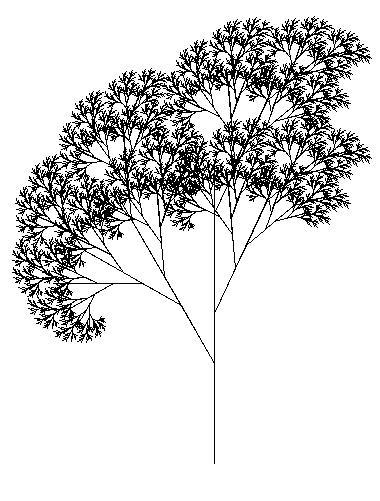
\includegraphics[width=\textwidth]{../images/RecursiveTree.JPG}
\end{minipage}
\end{footnotesize}
\end{frame}

\begin{frame}[fragile]
\begin{footnotesize}

  \headsp{Fakultetsfunktionen ($n!$)}

  En rekursiv definition:
  \vspace{-4mm}

  $$ \id{fac}(n) = \left \{ \begin{array}{lr} 1 & n \leq 1 \\ n*\id{fac}(n-1) & n > 1\end{array} \right . $$

    \head{En implementation i F\#:}

\begin{lstlisting}[numbers=none,frame=none,mathescape]
let rec fac n = if n <= 1 then 1
                else n * fac (n-1)
let x = fac 5

// = fac 5
// $\eval$ if 5 <= 1 then 1 else 5 * fac (5-1)
// $\eval$ if false then 1 else 5 * fac (5-1)
// $\eval$ 5 * fac (5-1) $\eval$ 5 * fac 4
// $\evals$ 5 * (4 * fac (4-1)) $\evals$ 5 * (4 * (3 * (2 * 1)))
// $\eval$ 5 * (4 * (3 * 2)) $\eval$ 5 * (4 * 6)
// $\eval$ 5 * 24 $\eval$ 120
\end{lstlisting}

\head{Bemærk:}
\begin{itemize}
\item Nøgleordet \lstinline{rec} er nødvendigt før en funktion kan henvise til sig selv...
\end{itemize}
\end{footnotesize}
\end{frame}

\newcommand{\addrRed}{{\tiny\id{\color{red}{0x23AF0$\bullet$}}}}
\newcommand{\addrTeal}{{\tiny\id{\color{teal}{0x9ABD0$\bullet$}}}}

\begin{frame}[fragile]
\begin{footnotesize}

  \headsp{Rekursion og funktionskald i F\#}

  Funktionskald håndteres med en \emph{kaldstak}, der benyttes til (1)
  at gemme indholdet af lokale variabler på tværs af kald samt (2) at
  overføre argumenter, returadresse og returværdi.

  \vspace{2mm}
  \begin{minipage}[t]{.64\textwidth}
  \textbf{Funktionskald:}

  \begin{enumerate}
  \item Returadresse og argumenter lægges på stakken.
  \item Der hoppes til funktionens adresse, hvor koden for funktionen er placeret.
  \item Funktionen køres og argumenter tilgås via stakken.
  \end{enumerate}

\vspace{1mm}
  \textbf{Funktionsreturnering:}

  \begin{enumerate}
  \item Argumenter og returadresse tages af stakken.
  \item Returværdi lægges på stakken.
  \item Der hoppes til returadressen.
  \item Kalder kan nu læse returværdien på stakken.
  \end{enumerate}

\vspace{1mm}
  \textbf{Bemærk:} Rekursion understøttes også med denne strategi (så længe stakken kan vokse ubegrænset).
  \end{minipage}
  \hspace{1mm}
  \begin{minipage}[t]{.34\textwidth}
    \vspace{-3mm}
    \textbf{Eksempel:} \lstinline[mathescape]{$\color{red}{\bullet}$fac 3} \\[2mm]
    $\begin{array}[b]{|p{10mm}|}\hline 3 \\ \hline \addrRed \\ \hline : \\ \hline \end{array}
    \eval
    \begin{array}[b]{|p{10mm}|}\hline 2 \\ \hline \addrTeal \\ \hline 3 \\ \hline \addrRed \\ \hline : \\ \hline \end{array}
    \cdots
    $ \\[5mm]
    $\begin{array}[b]{|p{10mm}|}\hline 3 $\times$ 2 \\ \hline \addrRed \\ \hline : \\ \hline \end{array}
    \eval
    \begin{array}[b]{|p{10mm}|}\hline 6 \\ \hline : \\ \hline \end{array}
    $ \\
    \vspace{-2mm}
\begin{lstlisting}[numbers=none,frame=none,mathescape]
let rec fac n =
  if n <= 1 then 1
  else n * $\color{teal}{\bullet}$fac(n-1)
let x =$\color{red}{\bullet}$fac 3
\end{lstlisting}
  \end{minipage}\hspace{-1cm}

\end{footnotesize}
\end{frame}

\begin{frame}[fragile]
\begin{footnotesize}

  \head{Fibonacci-tal}

  En rekursiv definition:

  $$ \id{fib}(n) = \left \{ \begin{array}{lr} 1 & n \in \{1,2\} \\ \id{fib}(n-1) + \id{fib}(n-2) & n > 2\end{array} \right . $$

    \head{En implementation i F\#:}

\begin{lstlisting}[numbers=none,frame=none,mathescape]
let rec fib n = if n = 1 || n = 2 then 1
                else fib (n-1) + fib (n-2)
let x = fib 5

// = fib 5
// $\evals$ fib(5-1) + fib(5-2) $\evals$ fib 4 + fib 3
// $\evals$ (fib(4-1) + fib(4-2)) + fib 3
// $\evals$ (fib 3 + fib 2) + fib 3
// $\evals$ ((fib 2 + fib 1) + fib 2) + fib 3 $\evals$ ((1 + 1) + 1) + fib 3
// $\evals$ 3 + (fib 2 + fib 1) $\evals$ 3 + (1 + 1) $\evals$ 5
\end{lstlisting}

\head{Bemærk:}
\begin{itemize}
\item De 10 første fibonacci tal: \lstinline{[1; 1; 2; 3; 5; 8; 13; 21; 34; 55]}
\end{itemize}
\end{footnotesize}
\end{frame}

%% \begin{frame}[fragile]
%% \begin{footnotesize}

%%   \head{Fibonacci-tal (forsat)}

%%   \head{Kald-træ:}

%%   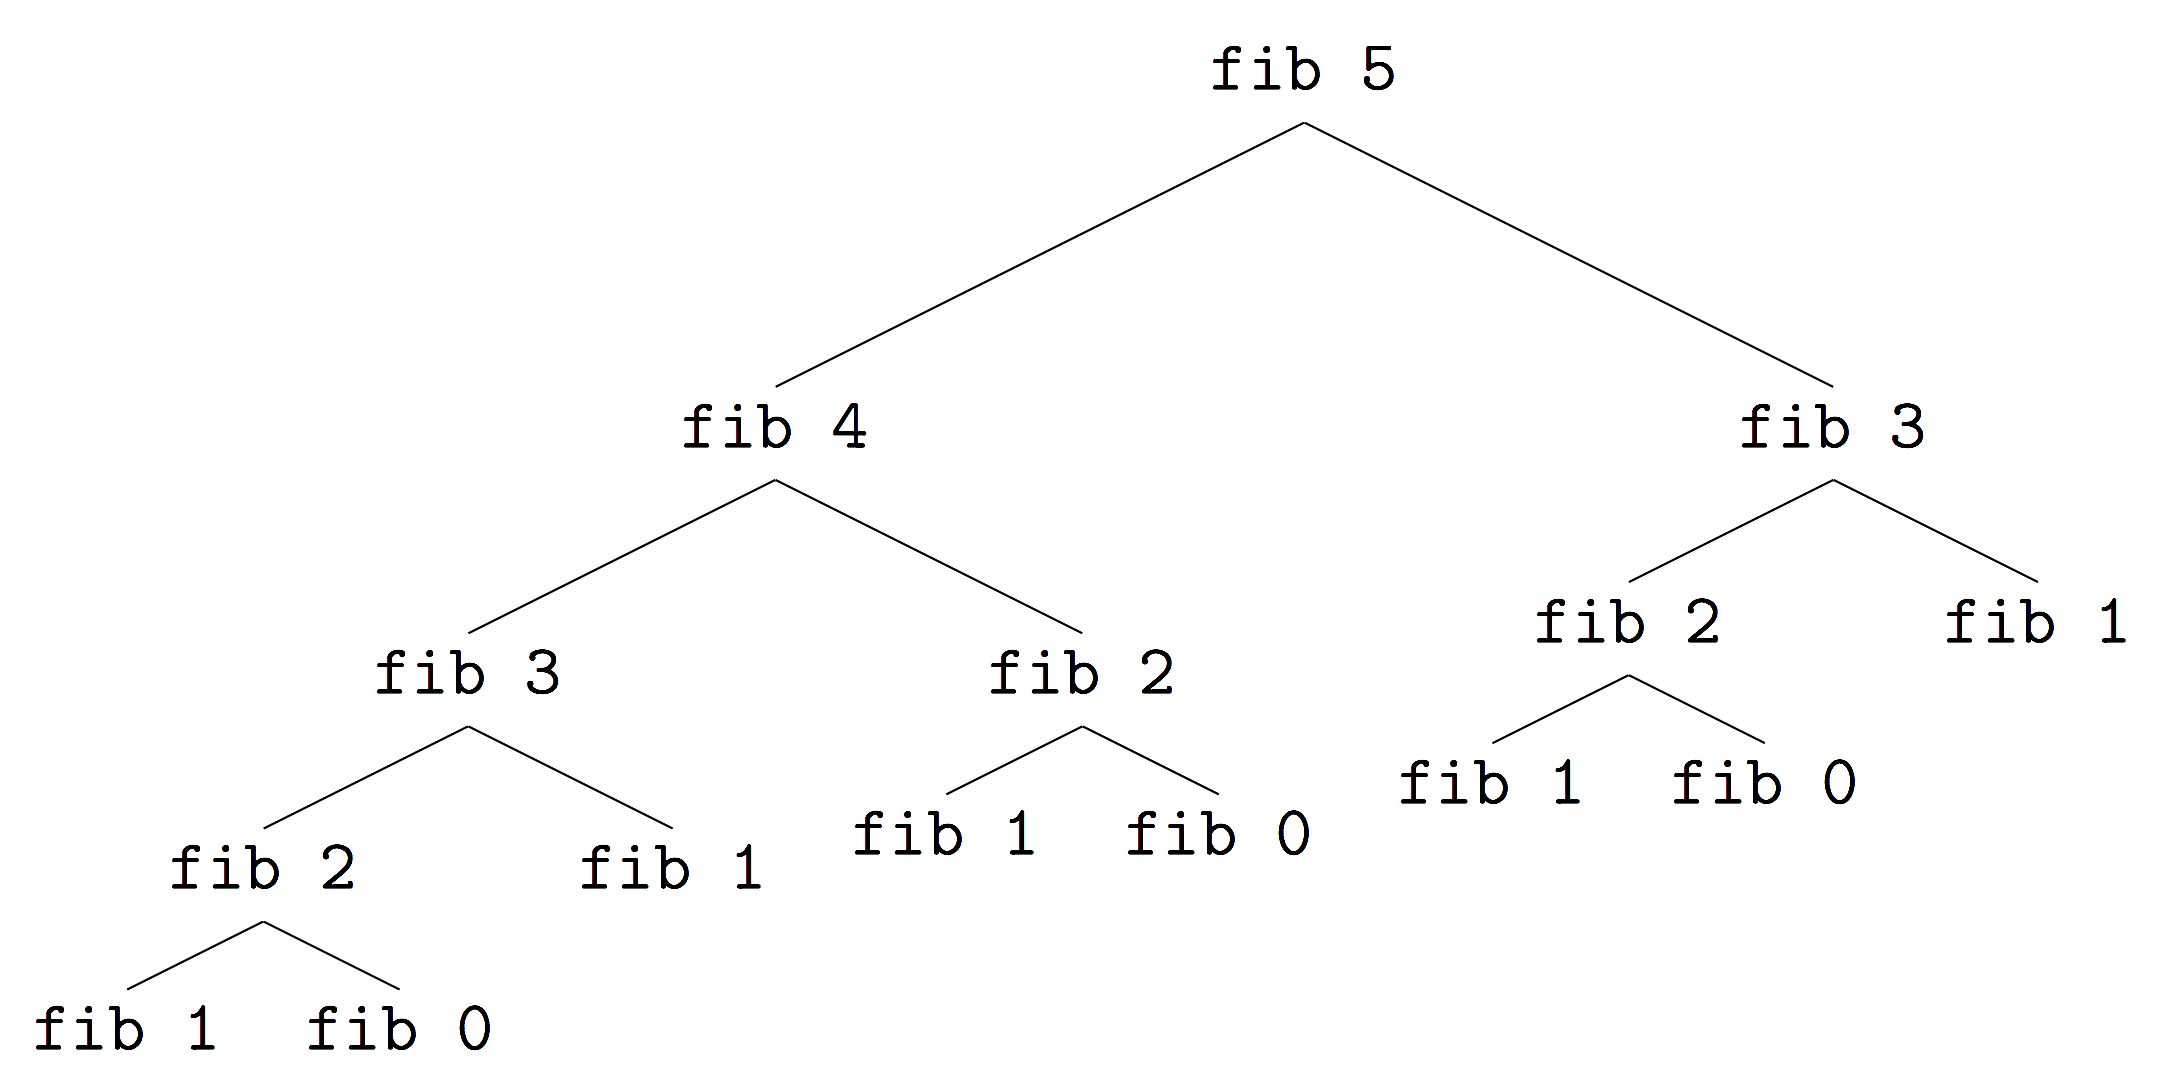
\includegraphics[width=0.9\textwidth]{../images/fib5.png}

%%   \head{Spørgsmål:}

%%   \begin{itemize}
%%     \item Kunne man forestille sig en hurtigere version af \lstinline{fib}?
%%   \end{itemize}
%% \end{footnotesize}
%% \end{frame}

\subsection{Halekald og halerekursion}

%% \begin{frame}[fragile]
%% \begin{footnotesize}

%%   \head{Fibonacci-tal (forsat)}

%%  \vspace{1ex}
%%   En mere effektiv implementation af fibonacci-tal i F\#:

%% \begin{lstlisting}[numbers=none,frame=none,mathescape]
%% let rec fib2 p1 p2 n =
%%   if n = 1 || n = 2 then p2
%%   else fib2 p2 (p1+p2) (n-1)

%% let xs = List.init 10 (fun x -> x + 1)
%% do printf "%A\n" (List.map (fib2 1 1) xs)
%% \end{lstlisting}

%% \head{Kørsel:}
%% \begin{verbatim}
%% bash-3.2$ fsharpc --nologo fib.fs && mono fib.exe
%% [1; 1; 2; 3; 5; 8; 13; 21; 34; 55]
%% \end{verbatim}

%% \head{Funktionen er ``hale-rekursiv''}

%% \begin{itemize}
%%   \item Efter det rekursive kald skal funktionen ikke foretage
%%     yderligere operationer for at fremkalde resultatet.
%%   \item Det betyder at funktionen kører i konstant stak-plads!
%% \end{itemize}

%% \end{footnotesize}
%% \end{frame}

\begin{frame}[fragile]
\begin{footnotesize}

  \headsp{Halekald}
  \vspace{1mm}

  Et funktionskald er et \emph{halekald} hvis resultatet af funktionskaldet umiddelbart returneres af kalderen (dvs: kaldet er det sidste gøremål).
  \vspace{2mm}
\begin{lstlisting}[numbers=none,frame=none,mathescape]
  let $\color{purple}\mathtt{f}$ x = $\color{red}\fbox{\texttt{g}}$ (... x ...)
\end{lstlisting}

  F\# implementerer halekald effektivt og \textbf{undgår unødig brug af
  stakplads} ved at sørge for at returadressen der er overført til {\color{purple}den
  kaldende funktion} sendes videre til den {\color{red}\fbox{kaldte funktion}} (således
  undgås også hop-til-hop).
  \vspace{2mm}

  Halekald i betingede udtryk implementeres som halekald hvis det
  betingede udtryk som et hele forkommer i en halekaldsposition.
  \vspace{2mm}
\begin{lstlisting}[numbers=none,frame=none,mathescape]
  let f x = if ... then ...
            else $\color{red}\fbox{\texttt{g}}$ ( ... x ... )
\end{lstlisting}

  \headsp{Halerekursion}

  \begin{minipage}{.42\textwidth}
  Hvis funktionen der kaldes er funktionen selv og kaldet er et
  halekald er der tale om \emph{halerekursion}.
  \end{minipage}
  \begin{minipage}{.55\textwidth}
\begin{lstlisting}[numbers=none,frame=none,mathescape]
  let rec $\color{purple}\fbox{\texttt{f}}$ x =
    if ... then ...
    else $\color{purple}\fbox{\texttt{f}}$ ( ... x ... )
\end{lstlisting}
  \end{minipage}
\end{footnotesize}
\end{frame}

\begin{frame}[fragile]
\begin{footnotesize}

  \head{Halerekursiv version af fakultetsfunktionen ($n!$)}

\begin{lstlisting}[numbers=none,frame=none,mathescape]
let rec hfac acc n =
  if n <= 1 then acc
  else hfac (n*acc) (n-1)

let x = hfac 1 5

// = hfac 1 5
// $\evals$ hfac (5*1) (5-1) $\evals$ hfac 5 4
// $\evals$ hfac (4*5) (4-1) $\evals$ hfac 20 3
// $\evals$ hfac (3*20) (3-1) $\evals$ hfac 60 2
// $\evals$ hfac (2*60) (2-1) $\evals$ hfac 120 1
// $\evals$ 120
\end{lstlisting}

\head{Bemærk:}

\begin{itemize}
\item Argumenter til en funktion evalueres til værdier før funktionen kaldes.
\item Der undgås en ``stak af ikke-udregnede udtryk'' (som i \lstinline[mathescape]{fac 5 $\evals$ 120}).
\item Brug halerekursion når det er oplagt muligt!
\end{itemize}

\end{footnotesize}
\end{frame}

%%%%%%%%%%%%%%%%%%%%%%%%%%%%%%%%%%%%%%%%%%%%%%%%
\subsection{Gensidig rekursion}
%%%%%%%%%%%%%%%%%%%%%%%%%%%%%%%%%%%%%%%%%%%%%%%%

\begin{frame}[fragile]
\begin{footnotesize}

  \head{Gensidig rekursion}

  \vspace{1ex}

  F\# tillader at man kan definere gensidigt rekursive funktioner.

  \head{Eksempel:}

  \vspace{1ex}

\begin{lstlisting}[numbers=none,frame=none,mathescape]
  let rec even x = if x = 0 then true
                   else odd (x-1)
  and odd x = if x = 0 then false
              else even (x-1)

  let t = not(odd 34) && even 36 && not(odd 0)
          && even 0 && not(even 1) && odd 1

  do printf "%b\n" t
\end{lstlisting}

\head{Bemærk:}
\begin{itemize}
\item Nøgleordet \lstinline{and} knytter de to gensidigt rekursive funktioner sammen.
\end{itemize}

\end{footnotesize}
\end{frame}

\subsection*{Konklusion}
\begin{frame}[fragile]
  \headsp{Konklusion}

  \vspace{3mm}
  \tableofcontents
\end{frame}
\end{document}

%%%%%%%%%%%%%%%%%%%%%%%%%%%%%%%%%%%%%%%%%%%%%%%%
\subsection{Rekursion over lister}
%%%%%%%%%%%%%%%%%%%%%%%%%%%%%%%%%%%%%%%%%%%%%%%%

\begin{frame}[fragile]
\begin{footnotesize}

  \head{Rekursion over Lister}

  \vspace{1ex}
  Vi kan finde længden på en liste ved hjælp af rekursion:
\begin{lstlisting}[numbers=none,frame=none,mathescape]
let rec length xs =
  if List.isEmpty xs then 0
  else 1 + length (List.tail xs)
\end{lstlisting}

\head{Bedre hale-rekursiv version (konstant stakplads)}
  \vspace{1ex}
\begin{lstlisting}[numbers=none,frame=none,mathescape]
let length xs =
  let rec len acc xs =
    if List.isEmpty xs then acc
    else len (acc+1) (List.tail xs)
  in len 0 xs
\end{lstlisting}

\head{Bemærk:}
\begin{itemize}
\item Vi vil senere se hvordan ``pattern-matching'' kan gøre definitionerne endnu mere læselige.
\end{itemize}
  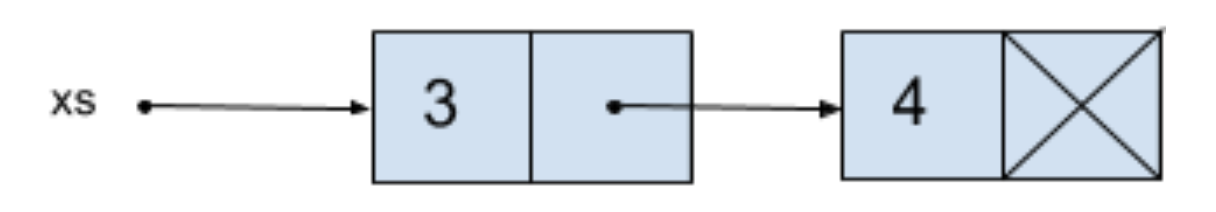
\includegraphics[width=0.5\textwidth]{../images/list34.png}

\end{footnotesize}
\end{frame}


\begin{frame}[fragile]
\begin{footnotesize}

  \head{Implementation af \lstinline{List.find} med rekursion}

  \vspace{1ex}
  Vi kan finde et element i en liste direkte ved hjælp af rekursion:
\begin{lstlisting}[numbers=none,frame=none,mathescape]
let rec find p xs =
  if List.isEmpty xs then None
  else if p (List.head xs) then Some (List.head xs)
       else find p (List.tail xs)

let xs = [34;23;56;76;23]

do printf "%A\n" (find (fun x -> x > 50) xs)
\end{lstlisting}

\head{De to rekursive tilfælde:}
  \vspace{1ex}
\begin{itemize}
\item Når listen er tom --- base case (\lstinline{[]}).
\item Når listen har mindst et element (\lstinline{::}).
\end{itemize}
  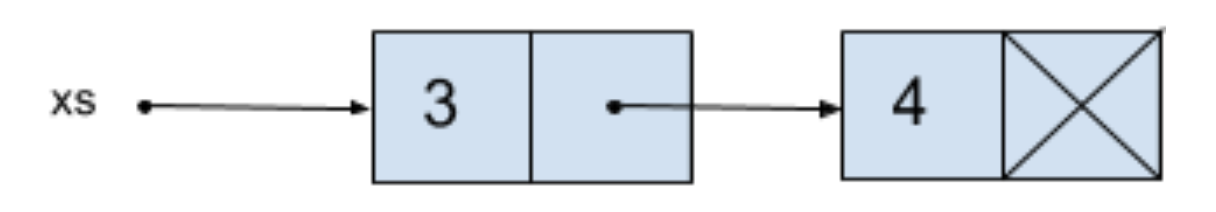
\includegraphics[width=0.5\textwidth]{../images/list34.png}

\end{footnotesize}
\end{frame}

%%%%%%%%%%%%%%%%%%%%%%%%%%%%%%%%%%%%%%%%%%%%%%%%
\subsection{Rekursion over arrays}
%%%%%%%%%%%%%%%%%%%%%%%%%%%%%%%%%%%%%%%%%%%%%%%%

\begin{frame}[fragile]
\begin{footnotesize}

  \head{Binær søgning i sorteret array}

  \vspace{1ex}
  Vi kan finde et element i et \textbf{sorteret} array hurtigere end ved at gennemløbe arrayet.

  \head{Binær søgning i array:}
\begin{lstlisting}[numbers=none,frame=none,mathescape]
let bsearch (arr:int[]) x =
  let rec bs min max =
       if min > max then None
       else let mid = (max+min) / 2
            in if x < arr.[mid] then bs min (mid-1)
               else if x > arr.[mid] then bs (mid+1) max
               else Some mid
  in bs 0 (Array.length arr - 1)

let arr = [|23;34;41;56;76;123;323|]   // sorteret array
do printf "%A\n" (bsearch arr 76)
\end{lstlisting}

\head{Kald af funktionen \lstinline{bs}:}
  \vspace{.5ex}
\begin{enumerate}
\item \lstinline{bs 0 7} $\eval$ \lstinline{mid} = 3
\item \lstinline{bs 4 7} $\eval$ \lstinline{mid} = 5  \hfill $\longleftarrow$ only $\id{log}(n)$ steps\ldots
\item \lstinline{bs 4 4} $\eval$ \lstinline{mid} = 4 $\eval$ Found
\end{enumerate}

\end{footnotesize}
\end{frame}


\end{document}
  - foundation
     sæt af heltal defineret rekursivt

  - factorial

  - fibonacci

  - even-odd

  - list length

  - list find

  - quick sort

  - merge sort

  - hanoi

  - tail-recursion

  - sierpienski

  - array binær søgning på sorteret data

  - array qsort


  \head{Repræsentationen af lister}

  \begin{itemize}
  \item Syntax:
\begin{lstlisting}[numbers=none,frame=none]
let lst = [1;2;3;4]
let lst2 = 5 :: List.tail (List.tail lst)
\end{lstlisting}

  \item Lagerrepræsentation:
    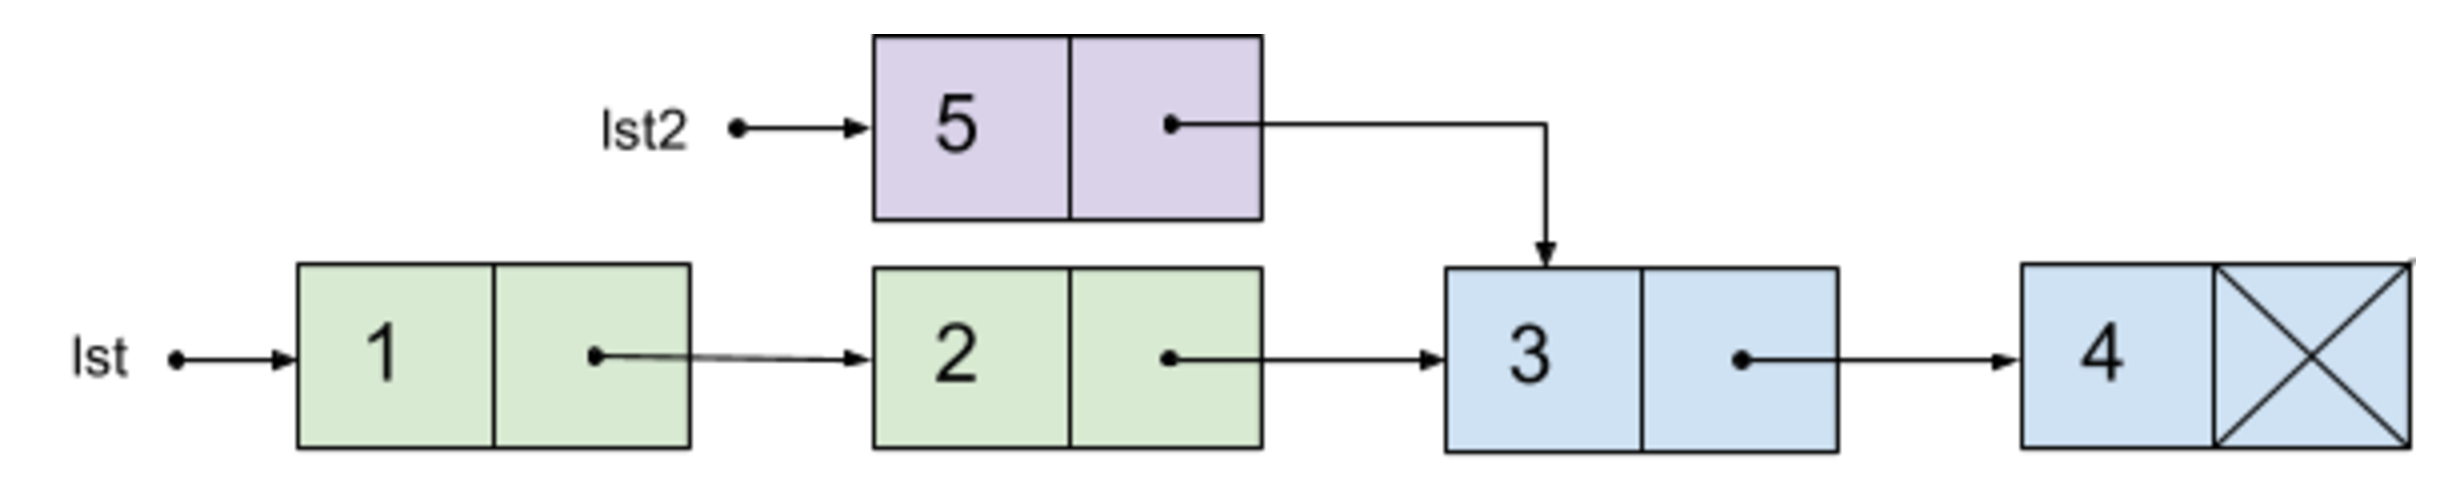
\includegraphics[width=0.9\textwidth]{list1234.png}

  \item Det er nemt at hægte et ekstra element på starten af en liste (\texttt{::}).

  \item Det er \textbf{IKKE} nemt (læs: hurtigt) at tilgå det sidste element i en liste.

  \item Lister er \emph{immutable}, dvs elementer kan ikke opdateres.

  \item Hvorfor kan immutabilitet være godt?
  \end{itemize}
\end{footnotesize}
\end{frame}

%%%%%%%%%%%%%%%%%%%%%%%%%%%%%%%%%%%%%%%%%%%%%%%%
\subsection{List modulet}
%%%%%%%%%%%%%%%%%%%%%%%%%%%%%%%%%%%%%%%%%%%%%%%%

\begin{frame}[fragile]
\begin{footnotesize}

\head{Modulet \lstinline{List}}

\vspace{1ex}

Modulet \lstinline{List} indeholder en lang række operationer på
lister.

\begin{lstlisting}[numbers=none,frame=none]
// list creation
val init     : int -> (int -> 'a) -> 'a list
val length   : 'a list -> int   // length l = l.Length

// list transformers
val map      : ('a -> 'b) -> 'a list -> 'b list
val map2     : ('a->'b->'c) -> 'a list -> 'b list -> 'c list
val filter   : ('a -> bool) -> 'a list -> 'a list

// list traversing
val fold     : ('s -> 'a -> 's) -> 's -> 'a list -> 's
val foldBack : ('a -> 's -> 's) -> 'a list -> 's -> 's
val find     : ('a -> bool) -> 'a list -> 'a option
...
\end{lstlisting}
\end{footnotesize}

\end{frame}


%%%%%%%%%%%%%%%%%%%%%%%%%%%%%%%%%%%%%%%%%%%%%%%%
\subsection{Beregninger på lister}
%%%%%%%%%%%%%%%%%%%%%%%%%%%%%%%%%%%%%%%%%%%%%%%%

\begin{frame}[fragile]
\begin{footnotesize}

  \head{Listefoldninger --- \lstinline{fold} og \lstinline{foldBack}}

  \vspace{1ex}

  Listefoldninger er generiske funktioner der gør det muligt at
  gennemløbe en liste for samtidig at foretage beregninger på
  elementerne, f.eks. for at opbygge en ny datastruktur.

  \vspace{1ex}

\begin{lstlisting}[numbers=none,frame=none,mathescape]
val fold     : ('s -> 'a -> 's) -> 's -> 'a list -> 's

 fold f s [x$_0$;x$_1$;x$_2$;...;x$_n$]
   = f ... (f (f (f s x$_0$) x$_1$) x$_2$) ... x$_n$

val foldBack : ('a -> 's -> 's) -> 'a list -> 's -> 's

 foldBack f [x$_0$;x$_1$;x$_2$;...;x$_n$] s
   = f x$_0$ (f x$_1$ (f x$_2$ ...(f x$_n$ s)...))
\end{lstlisting}

\end{footnotesize}
\end{frame}

\begin{frame}[fragile]
\begin{footnotesize}

\head{Eksempel: summation af elementerne i en liste}
\vspace{1ex}

\begin{lstlisting}[numbers=none,frame=none,mathescape]
let sum = List.fold (+) 0 [3;6;2;5]

//   = (((0 + 3) + 6) + 2) + 5
// $\eval$ ((3 + 6) + 2) + 5
// $\eval$ (9 + 2) + 5  $\eval$  11 + 5  $\eval$  16
\end{lstlisting}

\head{Eksempel: Find det mindste element i en liste}
\vspace{1ex}

\begin{lstlisting}[numbers=none,frame=none,mathescape]
let min x y = if x < y then x else y
let maxInt = System.Int32.MaxValue  // = 2147483647
let min_elem = List.fold min maxInt [3;6;2;5]

//   = min (min (min (min 2147483647 3) 6) 2) 5
// $\eval$ min (min (min 3 6) 2) 5
// $\eval$ min (min 3 2) 5  $\eval$  min 2 5  $\eval$  2
\end{lstlisting}

\head{Spørgsmål:}
\begin{enumerate}
\item Kunne man også have benyttet \lstinline{List.foldBack}?
\item Hvorfor tager \lstinline{List.fold} og \lstinline{List.foldBack} et initielt element?
\end{enumerate}

\end{footnotesize}
\end{frame}


\begin{frame}[fragile]
\begin{footnotesize}

\head{Eksempel: Det mindste element i en liste med \lstinline{List.foldBack}}
\vspace{1ex}

\begin{lstlisting}[numbers=none,frame=none,mathescape]
let min x y = if x < y then x else y
let maxInt = System.Int32.MaxValue  // = 2147483647
let min_elem = List.foldBack min maxInt [3;6;2;5]

// = min 3 (min 6 (min 2 (min 5 2147483647)))
// $\eval$ min 3 (min 6 (min 2 5))
// $\eval$ min 3 (min 6 2)
// $\eval$ min 3 2
// $\eval$ 2
\end{lstlisting}

\vspace{1ex}
\head{Funktionen \lstinline{min} er associativ og \lstinline{maxInt} er det neutrale element:}
\begin{enumerate}
\item For alle \lstinline{x}, \lstinline{y}, \lstinline{z}: \\ \lstinline{min x (min y z) = min (min x y) z}
\item For alle \lstinline{x}: \\ \lstinline{min 2147483647 x = min x 2147483647 = x}
\end{enumerate}

\end{footnotesize}
\end{frame}



\begin{frame}[fragile]
\begin{footnotesize}
  \head{Eksempel: Reverser en liste}
\vspace{1ex}

\begin{lstlisting}[numbers=none,frame=none,mathescape]
let f s x = x :: s
let rev xs = List.fold f [] xs

let ex = rev [1;2;3]

// = f (f (f [] 1) 2) 3
// $\eval$ f (f (1 :: []) 2) 3  $\eval$  f (2 :: 1 :: []) 3
// $\eval$ 3 :: 2 :: 1 :: []
\end{lstlisting}

\end{footnotesize}
\end{frame}

\begin{frame}[fragile]
\begin{footnotesize}
  \head{Eksempel: dot-produktet og vectorlængde}
\vspace{1ex}

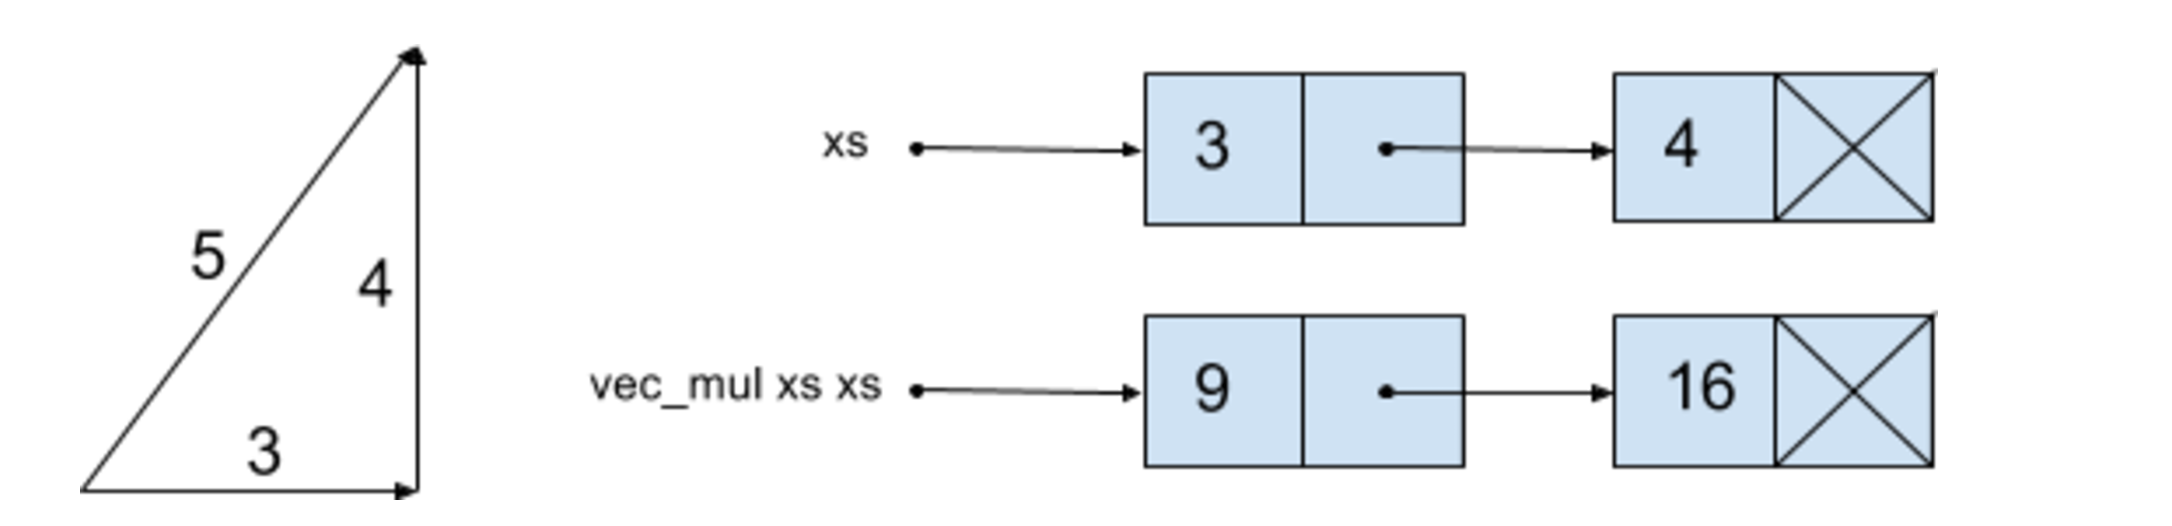
\includegraphics[width=0.9\textwidth]{vec345.png}

\begin{lstlisting}[numbers=none,frame=none,mathescape]
let vec_mul (xs:float list) ys = List.map2 (*) xs ys
let dot xs ys = List.fold (+) 0.0 (vec_mul xs ys)
let vec_len xs = sqrt (dot xs xs)
let ex = vec_len [3.0; 4.0]

// = sqrt (List.fold (+) 0.0 (vec_mul [3.0; 4.0] [3.0; 4.0]))
// $\evals$ sqrt (List.fold (+) 0.0 [9.0; 16.0])
// $\evals$ sqrt 25.0
// $\evals$ 5.0
\end{lstlisting}

\end{footnotesize}
\end{frame}

\begin{frame}[fragile]
\begin{footnotesize}
  \head{Funktionen \lstinline{List.find}}
\vspace{1ex}

\begin{lstlisting}[numbers=none,frame=none,mathescape]
val find : ('a -> bool) -> 'a list -> 'a option
\end{lstlisting}

Udtrykket (\lstinline{find p xs}) returnerer (\lstinline{Some x}) hvis
\lstinline{x} er det første element i \lstinline{xs} for hvilket
(\lstinline{p x}) evaluerer til \lstinline{true}. Udtrykket returnerer
\lstinline{None} hvis der ikke findes et sådan element.

\vspace{1ex}
\head{Implementation af \lstinline{List.find} ved brug af \lstinline{List.fold}}
\vspace{1ex}

\begin{lstlisting}[numbers=none,frame=none,mathescape]
let find p xs =
  List.fold (fun s x -> if s = None && p x then Some x else s)
            None xs

// find (fun x -> x > 4) [3;2;5;6;45]
// $\evals$ 5
\end{lstlisting}

\end{footnotesize}
\end{frame}

\begin{frame}[fragile]
\begin{footnotesize}
\head{For-in løkker---et alternativ til \lstinline{List.fold}}

\vspace{2ex}

Et alternativ til \lstinline{List.fold} er at benytte den specielle
\lstinline{for-in-do} syntax til liste-gennemløb:

\vspace{1ex}

\begin{lstlisting}[numbers=none,frame=none,mathescape]
let lst = List.init 50000 (fun x -> x)
let mutable sum = 0
for x in lst do sum <- sum + x
do printf "%d\n" sum
\end{lstlisting}

\vspace{1ex}

\head{Fordele:}
\begin{enumerate}
\item Ingen overhead ved liste-indicering eller kald til \lstinline{lst.Length}.
\item Simplere form for imperativ programmering; dog er \lstinline{sum} stadig mutable...
\end{enumerate}
\end{footnotesize}
\end{frame}

%%%%%%%%%%%%%%%%%%%%%%%%%%%%%%%%%%%%%%%%%%%%%%%%
\section{Programmering med Arrays}
%%%%%%%%%%%%%%%%%%%%%%%%%%%%%%%%%%%%%%%%%%%%%%%%


%%%%%%%%%%%%%%%%%%%%%%%%%%%%%%%%%%%%%%%%%%%%%%%%
\subsection{1D Arrays}
%%%%%%%%%%%%%%%%%%%%%%%%%%%%%%%%%%%%%%%%%%%%%%%%

\begin{frame}[fragile]
\begin{footnotesize}
  \head{Repræsentationen af arrays}

  \begin{itemize}
  \item Syntax:
\begin{lstlisting}[numbers=none,frame=none]
let arr = [|1;2;3;4|]
\end{lstlisting}

  \item Lagerrepræsentation: \\
    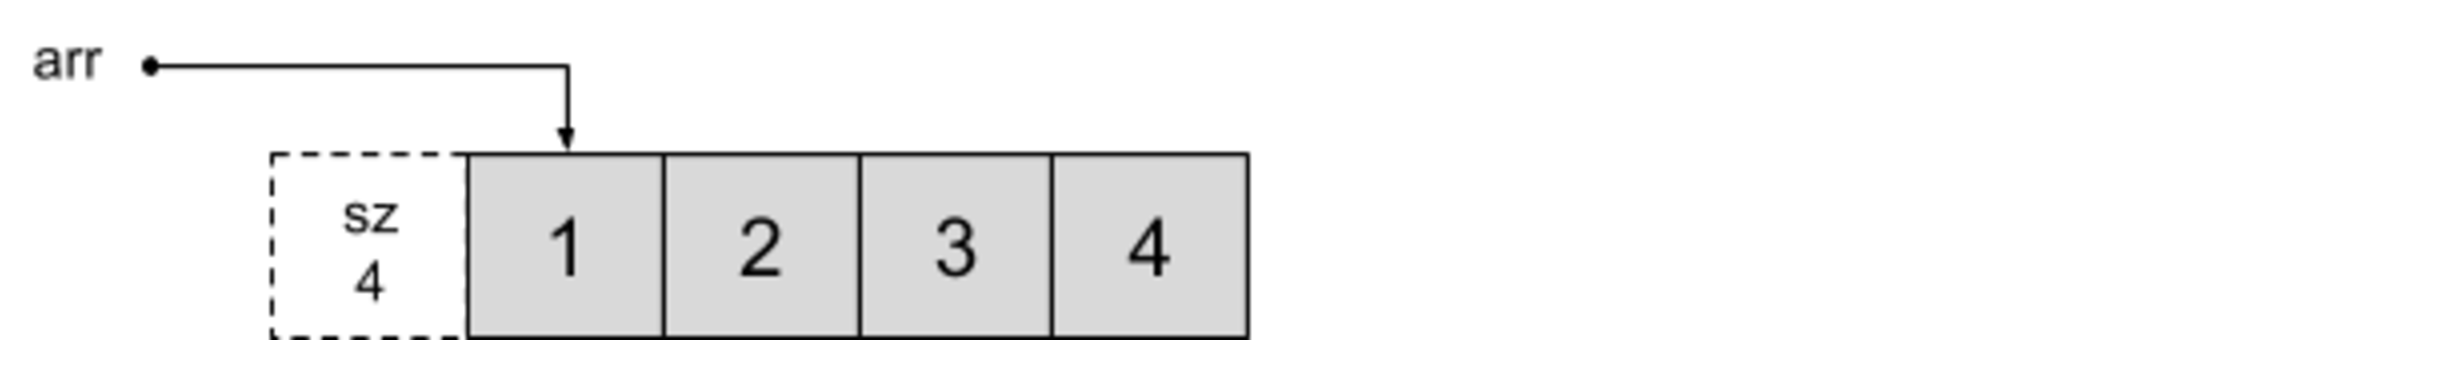
\includegraphics[width=0.9\textwidth]{array1234.png}
  \item Det er \textbf{IKKE} nemt at tilføje ekstra elementer.
  \item Det er nemt (hurtigt) at læse ethvert element i et array.

  \item Arrays er \emph{mutable}, dvs det er muligt (hurtigt) at
    opdatere ethvert element.
  \item Typen for integer arrays: \lstinline{int[]}
  \item Typen for arrays indeholdende int-float par: \lstinline{(int*float)[]}
  \end{itemize}
\end{footnotesize}
\end{frame}

\begin{frame}[fragile]
\begin{footnotesize}
\head{Gennemløb af arrays}

\vspace{1ex}

Arrays kan gennemløbes tilsvarende som lister:

\vspace{1ex}

\begin{lstlisting}[numbers=none,frame=none,mathescape]
let arr = Array.init 50000 (fun x -> x)
let mutable sum = 0
for x in arr do sum <- sum + x
do printf "%d\n" sum
\end{lstlisting}

\vspace{1ex}
\head{Arrays kan muteres:}
\vspace{1ex}

\begin{lstlisting}[numbers=none,frame=none,mathescape]
let arr = [|1;2;3;4|]
for i in [0..arr.Length-1] do arr.[i] <- arr.[i]*arr.[i]
do printf "%A\n" arr
\end{lstlisting}

\vspace{1ex}
\head{Kørsel:}

\begin{verbatim}
bash-3.2$ fsharpc --nologo arr_square.fs && mono arr_square.exe
[|1; 4; 9; 16|]
\end{verbatim}
\end{footnotesize}
\end{frame}


\begin{frame}[fragile]
\begin{footnotesize}
\head{Array aliasing}

\vspace{1ex}

To forskellige variabler kan referere til det samme array:
\begin{lstlisting}[numbers=none,frame=none,mathescape]
let arr = [|1;2;3;4|]
let b = arr
do b[1] <- 100
do printf "%A\n" arr
\end{lstlisting}

\vspace{1ex}
\head{Lagerrepræsentation:}
\vspace{1ex}

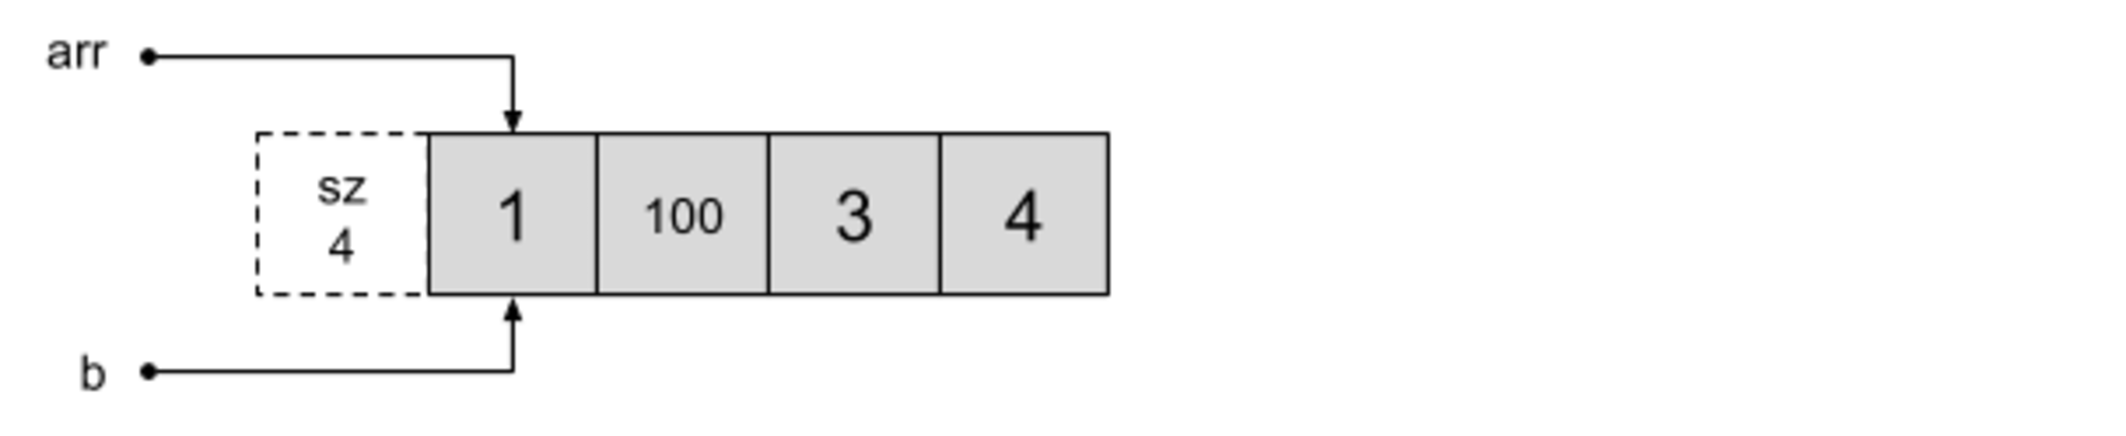
\includegraphics[width=0.9\textwidth]{arr_b_1234.png}

\vspace{1ex}
\head{Bemærk:}
\begin{enumerate}
\item Aliasing kan observeres fordi arrays er mutable!
\item Aliasing (og deling) kan ikke observeres (på samme måde) med lister, da disse er immutable.
\end{enumerate}

\end{footnotesize}
\end{frame}

\begin{frame}[fragile]
\begin{footnotesize}
\head{Modulet \lstinline{Array}}
\vspace{1ex}
\begin{lstlisting}[numbers=none,frame=none]
// array creation
val init     : int -> (int -> 'a) -> 'a []
val length   : 'a [] -> int   // length a = a.Length
val toList   : 'a [] -> 'a list
val ofList   : 'a list -> 'a []

// array transformers
val map      : ('a -> 'b) -> 'a [] -> 'b []
val map2     : ('a->'b->'c) -> 'a [] -> 'b [] -> 'c []
val filter   : ('a -> bool) -> 'a [] -> 'a []

// array traversing
val fold     : ('s -> 'a -> 's) -> 's -> 'a [] -> 's
val foldBack : ('a -> 's -> 's) -> 'a [] -> 's -> 's
val find     : ('a -> bool) -> 'a [] -> 'a option
...
\end{lstlisting}

\end{footnotesize}
\end{frame}


%%%%%%%%%%%%%%%%%%%%%%%%%%%%%%%%%%%%%%%%%%%%%%%%
\subsection{2D Arrays}
%%%%%%%%%%%%%%%%%%%%%%%%%%%%%%%%%%%%%%%%%%%%%%%%

\begin{frame}[fragile]
\begin{footnotesize}
\head{To-dimensionelle arrays}
\vspace{1ex}

To-dimensionelle \emph{regulære arrays}, dvs. 2d-arrays hvor alle
rækker indeholder det samme antal elementer, kan udtrykkes ved brug af
modulet \lstinline{Array2D}.

\vspace{1ex}

Modulet \lstinline{Array2D} kan benyttes til f.eks. at konstruere
en multiplikationstabel:

\vspace{1ex}

\begin{lstlisting}[numbers=none,frame=none]
let a = Array2D.init 5 5 (fun r c -> (r+1) * (c+1))
let prA (a : int[,]) =
  for r in [0..Array2D.length1 a - 1] do    // 1  2  3  4  5
    for c in [0..Array2D.length2 a - 1] do  // 2  4  6  8 10
      printf "%2d " (a.[r,c])               // 3  6  9 12 15
    printf "\n"                             // 4  8 12 16 20
do prA a                                    // 5 10 15 20 25
\end{lstlisting}

\head{Bemærk:}
\vspace{1ex}

\begin{enumerate}
\item Typen på et to-dimensionelt int-array skrives: \lstinline{int[,]}.
\item Vidden på de udskrevne heltal kontrolleres med format-specifieren \lstinline{"%2d "}.
\end{enumerate}
\end{footnotesize}
\end{frame}


\end{document}
